\documentclass[11pt]{article}
\usepackage[margin=0.6in]{geometry}
\usepackage[T1]{fontenc}
\usepackage{lmodern}
\usepackage{tikz}
\usetikzlibrary{positioning,arrows.meta}
\usepackage{booktabs}
\usepackage{array}
\usepackage{hyperref}
\pagestyle{empty}
\begin{document}

\section*{Study Selection Demonstration for Replication}

\noindent\textbf{Important note.} For the sake of replication, this package demonstrates the screening trace most concretely with the \textbf{802-study title/abstract pool}, because this is the subset directly backed by the narrowed metadata and record-level screening decisions included in the package. This \textbf{802-study trace is only a demonstration subset}. The \textbf{actual study} reported in the manuscript began with \textbf{4,010 initial records} and ended with \textbf{107 final primary studies}.\medskip

\begin{table}[h!]
\centering
\small
\begin{tabular}{>{\raggedright\arraybackslash}p{0.52\textwidth} >{\centering\arraybackslash}p{0.12\textwidth} >{\raggedright\arraybackslash}p{0.25\textwidth}}
\toprule
\textbf{Stage} & \textbf{Count} & \textbf{Meaning} \\
\midrule
Initial retrieval & 4,010 & Records retrieved from IEEE Xplore, ACM, SpringerLink, ScienceDirect, and Google Scholar \\
After deduplication and short-paper filtering & 2,406 & Duplicates and records under the page-length criterion removed \\
Title/abstract screening pool & 802 & Metadata-backed replication demonstration begins here \\
After introduction/conclusion screening & 267 & Narrowed to records sufficiently related to fairness requirements / AI systems \\
Database-screened set after full-text assessment & 107 & Retained from the database-screened branch before snowballing integration \\
Snowballing additions & 30 & Additional studies brought in through backward/forward snowballing \\
QA/integration pool & 137 & Combined set assessed before final corpus freeze \\
Final primary studies & 107 & Final analytical corpus used in the review \\
\bottomrule
\end{tabular}
\end{table}

\begin{figure*}[t]
\centering
\resizebox{0.95\textwidth}{!}{%
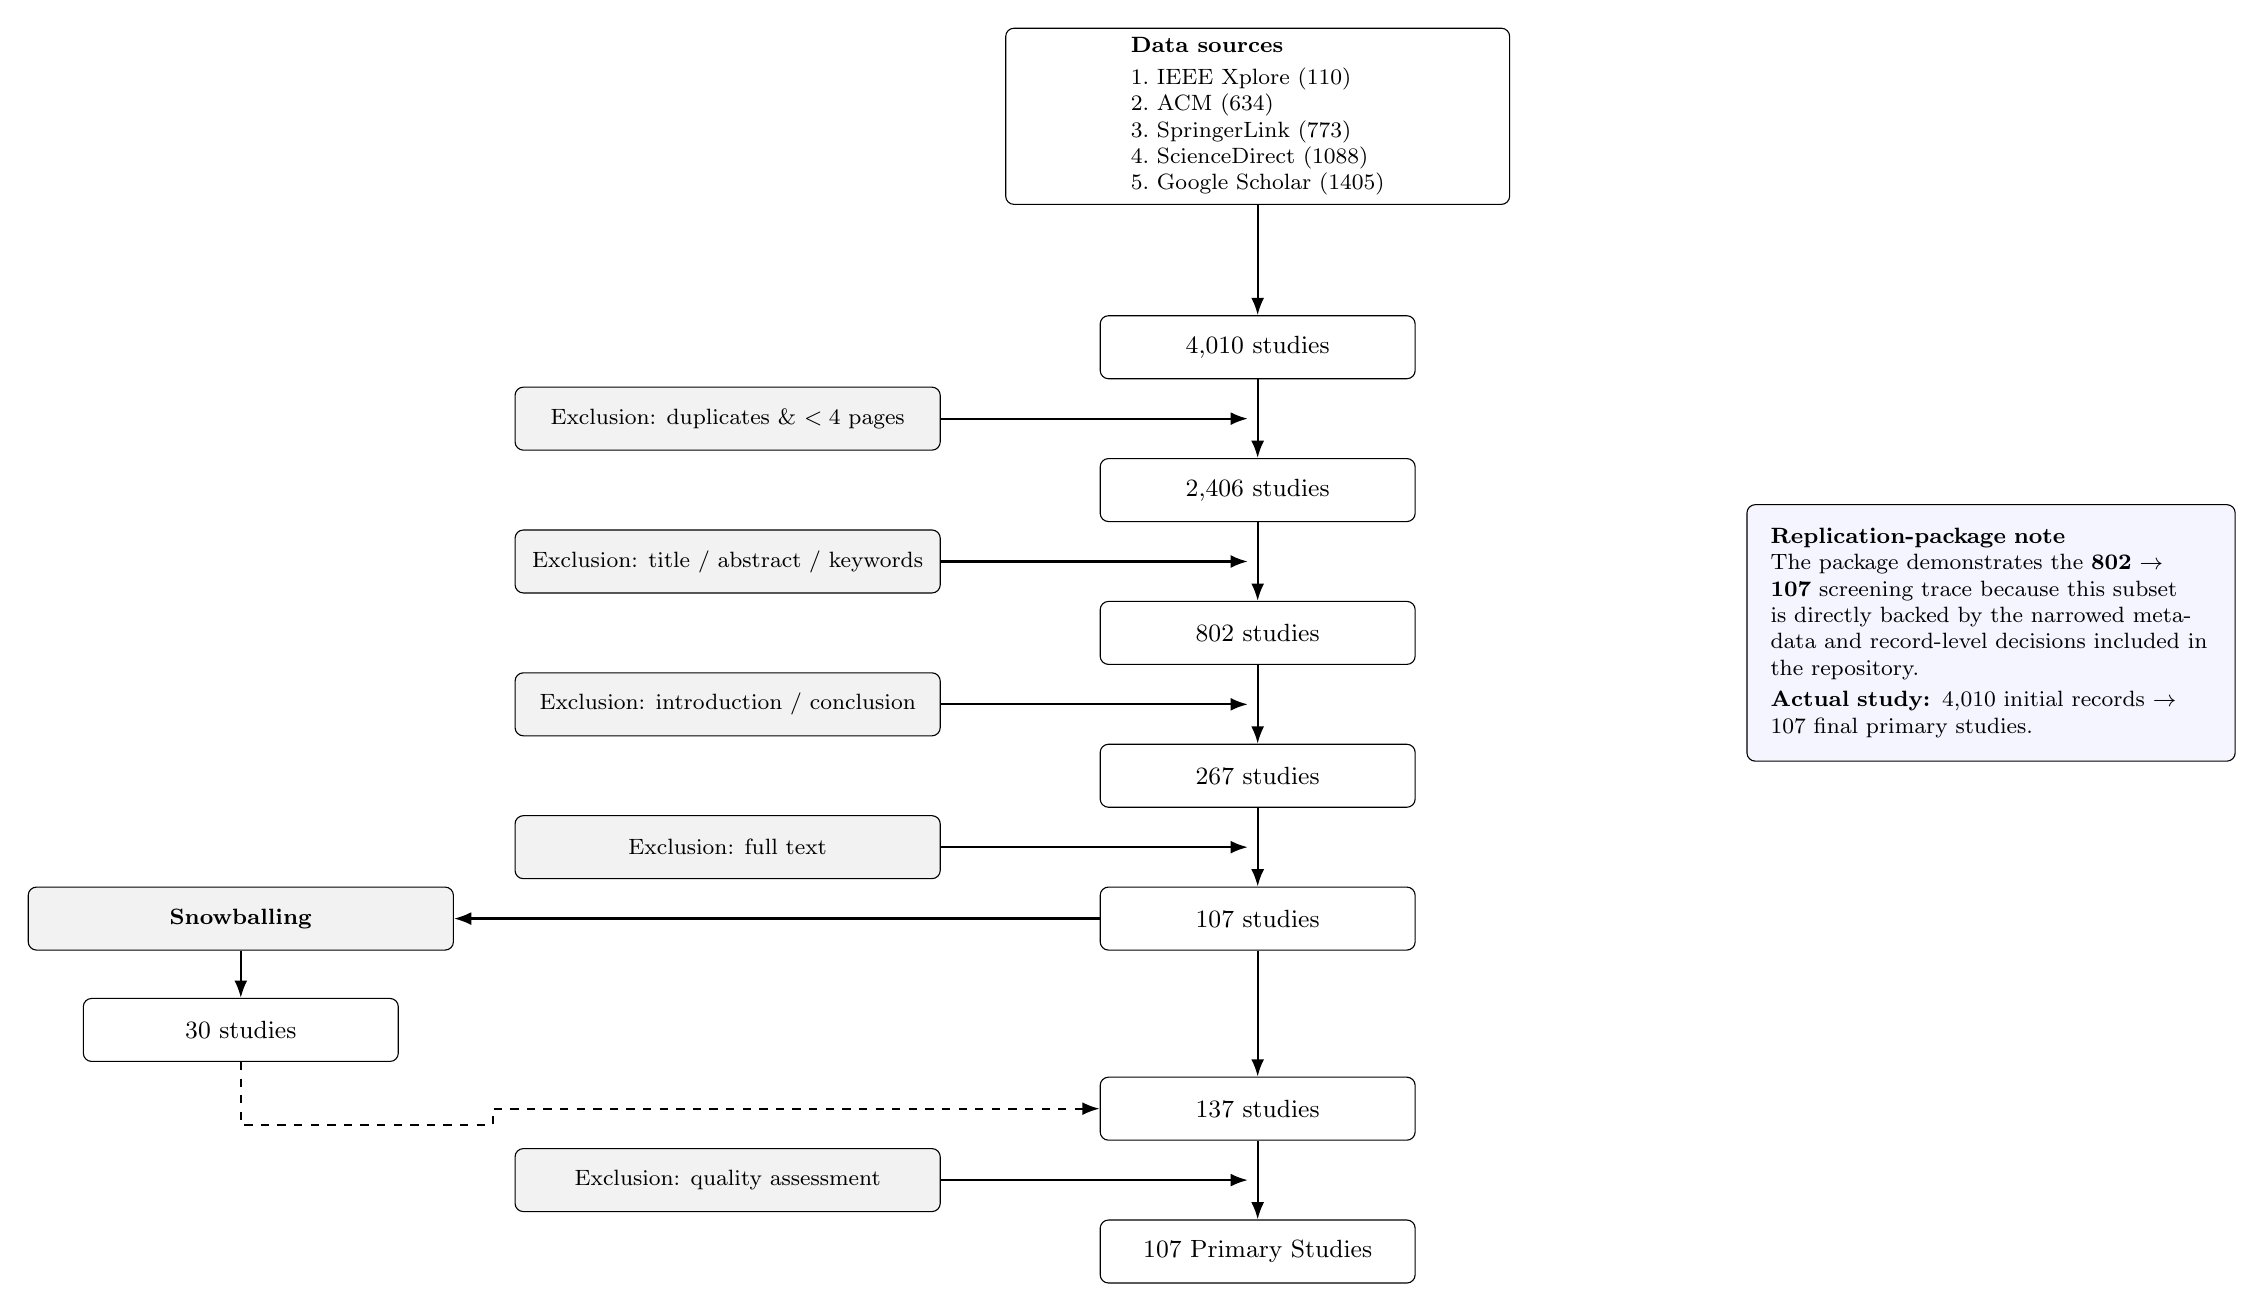
\begin{tikzpicture}[
    font=\small,
    node distance=10mm and 18mm,
    >={Latex[length=2.2mm]},
    line/.style={->, thick},
    stage/.style={
        draw, rounded corners=3pt,
        minimum width=40mm,
        minimum height=8mm,
        align=center
    },
    excl/.style={
        draw, rounded corners=3pt,
        fill=gray!10,
        minimum width=54mm,
        minimum height=8mm,
        align=center,
        font=\footnotesize
    },
    source/.style={
        draw, rounded corners=3pt,
        align=left,
        font=\footnotesize,
        minimum width=64mm
    },
    note/.style={
        draw, rounded corners=3pt,
        fill=blue!4,
        align=left,
        font=\footnotesize,
        text width=56mm,
        inner sep=3mm
    }
]

% Sources
\node[source] (sources) {%
\textbf{Data sources}\\[2pt]
1.\ IEEE Xplore (110)\\
2.\ ACM (634)\\
3.\ SpringerLink (773)\\
4.\ ScienceDirect (1088)\\
5.\ Google Scholar (1405)
};

% Main chain
\node[stage, below=14mm of sources] (s4010) {4,010 studies};
\node[stage, below=of s4010]        (s2406) {2,406 studies};
\node[stage, below=of s2406]        (s802)  {802 studies};
\node[stage, below=of s802]         (s267)  {267 studies};
\node[stage, below=of s267]         (s107db){107 studies};
\node[stage, below=16mm of s107db]  (s137)  {137 studies};
\node[stage, below=of s137]         (s107)  {107 Primary Studies};

% Main arrows
\draw[line] (sources.south) -- (s4010.north);
\draw[line] (s4010.south)  -- (s2406.north);
\draw[line] (s2406.south)  -- (s802.north);
\draw[line] (s802.south)   -- (s267.north);
\draw[line] (s267.south)   -- (s107db.north);
\draw[line] (s107db.south) -- (s137.north);
\draw[line] (s137.south)   -- (s107.north);

% Midpoints
\path (s4010) -- (s2406) node[midway] (mid4010_2406) {};
\path (s2406) -- (s802)  node[midway] (mid2406_802)  {};
\path (s802)  -- (s267)  node[midway] (mid802_267)   {};
\path (s267)  -- (s107db) node[midway] (mid267_107)  {};
\path (s137)  -- (s107)  node[midway] (mid137_107)   {};

% Exclusion boxes
\node[excl, left=39mm of mid4010_2406] (eDup)
  {Exclusion: duplicates \& $<4$ pages};
\node[excl, left=39mm of mid2406_802] (eTitle)
  {Exclusion: title / abstract / keywords};
\node[excl, left=39mm of mid802_267] (eIntro)
  {Exclusion: introduction / conclusion};
\node[excl, left=39mm of mid267_107] (eFull)
  {Exclusion: full text};
\node[excl, left=39mm of mid137_107] (eQual)
  {Exclusion: quality assessment};

\draw[line] (eDup.east)   -- (mid4010_2406.west);
\draw[line] (eTitle.east) -- (mid2406_802.west);
\draw[line] (eIntro.east) -- (mid802_267.west);
\draw[line] (eFull.east)  -- (mid267_107.west);
\draw[line] (eQual.east)  -- (mid137_107.west);

% Snowballing branch
\node[excl, left=82mm of s107db] (snow) {\textbf{Snowballing}};
\node[stage, below=6mm of snow] (s30) {30 studies};
\draw[line] (s107db.west) -- ++(-8mm,0) |- (snow.east);
\draw[line] (snow.south) -- (s30.north);
\draw[line, dashed] (s30.south) -- ++(0,-8mm) -- ++(32mm,0) |- (s137.west);

% Package note on the right
\node[note, right=42mm of s802] (pkgNote) {\textbf{Replication-package note}\\
The package demonstrates the \textbf{802 $\rightarrow$ 107} screening trace because this subset is directly backed by the narrowed metadata and record-level decisions included in the repository.\\[2pt]
\textbf{Actual study:} 4,010 initial records $\rightarrow$ 107 final primary studies.};

\end{tikzpicture}%
}
\caption{Study selection and screening process for identifying primary studies. For the sake of replication, the package demonstrates the metadata-backed \textbf{802-to-107} segment in an inspectable way. This is a \textbf{demonstration subset only}: the actual study began with \textbf{4,010 initial records} and concluded with \textbf{107 final primary studies}.}
\label{fig:study-selection-demonstration}
\end{figure*}

\end{document}
